%%% Laboratory	 Notes
%%% Template by Mikhail Klassen, April 2013
%%% Contributions from Sarah Mount, May 2014
\documentclass[a4paper]{tufte-handout}
\usepackage{tikz}

\newcommand{\workingDate}{\textsc{April $|$ 2022}}
\newcommand{\userName}{A.Belcaid}
\newcommand{\institution}{ENSA-Safi}

\usepackage{lab_notes}

\usepackage{hyperref}
\hypersetup{
    pdffitwindow=false,            % window fit to page
    pdfstartview={Fit},            % fits width of page to window
    pdftitle={Correction TD4},     % document title
    pdfauthor={A.Belcaid},         % author name
    pdfsubject={},                 % document topic(s)
    pdfnewwindow=true,             % links in new window
    colorlinks=true,               % coloured links, not boxed
    linkcolor=DarkScarletRed,      % colour of internal links
    citecolor=DarkChameleon,       % colour of links to bibliography
    filecolor=DarkPlum,            % colour of file links
    urlcolor=DarkSkyBlue           % colour of external links
}


\title{Solution TD 6}
\date{2022}

\begin{document}
\maketitle

\renewcommand{\P}{\mathbf{P}}

\section{Loi de probabilite}

Pour que $\P_X$ definit une loi de probabilite il faut que:

\begin{eqnarray*}
1& = & \sum_x \P_x(x) \\
1 & = & \P_x(-3) + \P_x(-2) + \P_x(-1) + \P_x(3) + \P_x(2) + \P_x(1)\\
               1 & = & 2\left(\frac{9}{a}\right) + 2\left(\frac{4}{a}\right) +
               2\left(\frac{1}{a}\right)\\
                 & = & \frac{28}{a}
\end{eqnarray*}
Ainsi 
$$
a = 28
$$.
\begin{marginfigure}
\begin{center}
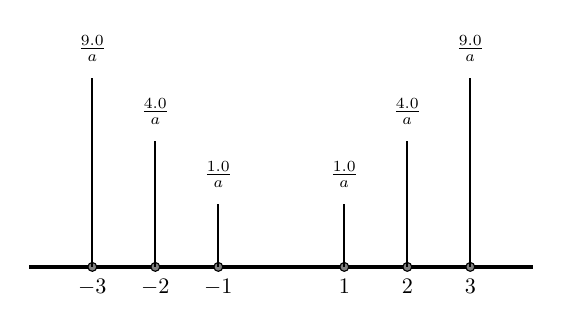
\begin{tikzpicture}[scale=.8, transform shape]
  \path[draw,-,very thick] (-4,0) -- (4,0);
   \foreach \x in {-3, -2, -1, 1, 2, 3}
   { 
     \node[draw, fill=gray, minimum width=4pt, circle, inner sep=0pt,
       label=below:$\x$] at (\x, 0) {};
     \pgfmathsetmacro\ax{abs(\x)}
     \pgfmathsetmacro\xx{pow(\x,2)}
     \path[draw, thick] (\x,0) -- (\x, \ax)node[label=above:{$\frac{\xx}{a}$}]{};
     
   }
\end{tikzpicture}
\end{center}
\caption{Loi de $X$}%
\end{marginfigure}

Soit $Z = X^2$, on cherche la loi de probabilite de $Z$.
  On a:
  \begin{equation*}
    \P_Z(k) = \P_X(x^2 = k)
  \end{equation*}
  Ainsi l'ensembles des valeurs $k$ que peut prendre $Z$ est $\left\{1, 4,
  9\right\}.$

  On obtient alors:

  \begin{equation*}
    P_Z(k) = \begin{cases}
      \frac{2}{28}    & k = 1\\[4pt]
      \frac{4}{28}    & k = 4\\[4pt]
      \frac{18}{28}    & k = 9\\[4pt]
    \end{cases}
  \end{equation*}
\begin{marginfigure}
\begin{center}
\begin{tikzpicture}[scale=0.5]
  \path[draw,-,very thick] (-0,0) -- (10,0);
   \foreach \x/\y in {1/1, 4/4, 9/18}
   { 
     \node[draw, fill=gray, minimum width=4pt, circle, inner sep=0pt,
       label=below:$\x$] at (\x, 0) {};
     \pgfmathsetmacro\ax{abs(\x)}
     \pgfmathsetmacro\xx{2*\x}
     \path[draw, thick] (\x,0) -- (\x, \ax)node[label=above:{$\frac{\xx}{a}$}]{};
     
   }
\end{tikzpicture}
\end{center}
\caption{Loi de $Z$}%
\end{marginfigure}

\section{Loi d'un de truque}
La variables $X$ prend des valeurs dans $\left\{1,2,\ldots,6\right\}$. Par
hypothese, il existe un reel $a$ tel que 

$$
 \P_X(k) = ka
$$

Ce reel doit verifier la relation:

\begin{eqnarray}
  \sum_{x=1}^6 \P_X(x) &=& 1\\ 
  a \times \left(\frac{6\times 7}{2}\right) & = & 1\\
  \frac{21}{a}  & = & 1
\end{eqnarray}
D'ou $ \mathbf{a} = \frac{1}{21}$

On obtient ainsi la loi suivante:

\begin{table}[htpb]
  \centering
  \caption{ Loi de distribution du de}

  \begin{array}{ccccccc}
    \toprule
    k & 1 & 2 & 3 & 4 & 5 & 6\\[4pt]
    \midrule
    \P_X(x=k) & \frac{1}{21}& \frac{2}{21} & \frac{3}{21} & \frac{4}{21} &
    \frac{5}{21} & \frac{6}{21}\\[4pt]
    \bottomrule
  \end{array} 
\end{table}

Calculons maintenant l'\textbf{esperance} de $X$.

\begin{eqnarray*}
  \mathbf{E}[X] &=& \sum_{x=1}^6 x\P_X(x)\\
                &=& \frac{1}{21} \sum_{x=1}^6 x^2\\
                &=& \frac{91}{21}\\
                &=& \frac{13}{3}
\end{eqnarray*}

Soit $Y$ une variable definie par $\frac{1}{X}$. Alors la loi de $Y$ est donne
par:

\begin{table}[htpb]
  \centering
  \caption{Loi de probaiblite de $Y$}
  \label{tab:label}
  
  \begin{array}{ccccccc}
    \toprule
    \frac{1}{k} & \frac{1}{1} & \frac{1}{2} & \frac{1}{3} & \frac{1}{4} &
    \frac{1}{5} & \frac{1}{6}\\[4pt]
    \midrule
    \P_Y(=k) & \frac{1}{21}& \frac{2}{21} & \frac{3}{21} & \frac{4}{21} &
    \frac{5}{21} & \frac{6}{21}\\[4pt]
    \bottomrule

  \end{array}
\end{table}

Si on calcule l'esperance de $Y$, on trouve:
\begin{equation}
  \mathbf{E}(Y) = \frac{2}{7}
\end{equation}

Le but est d'introduire aux etudiantes l'erreur classique que 
$$
\mathbf{E}(g(X))  \neq g(\mathbbf{E}(X))
$$
\end{document}


